% Created 2022-03-12 Sat 10:22
% Intended LaTeX compiler: pdflatex
\documentclass[11pt]{article}
\usepackage[utf8]{inputenc}
\usepackage[T1]{fontenc}
\usepackage{graphicx}
\usepackage{longtable}
\usepackage{wrapfig}
\usepackage{rotating}
\usepackage[normalem]{ulem}
\usepackage{amsmath}
\usepackage{amssymb}
\usepackage{capt-of}
\usepackage{hyperref}
\usepackage{minted}
\graphicspath{{../../books/}}
% TIPS
% \substack{a\\b} for multiple lines text





% pdfplots will load xolor automatically without option
\usepackage[dvipsnames]{xcolor}

\usepackage{forest}
% two-line text in node by [two \\ lines]
% \begin{forest} qtree, [..] \end{forest}
\forestset{
  qtree/.style={
    baseline,
    for tree={
      parent anchor=south,
      child anchor=north,
      align=center,
      inner sep=1pt,
    }}}
%\usepackage{flexisym}
% load order of mathtools and mathabx, otherwise conflict overbrace

\usepackage{mathtools}
%\usepackage{fourier}
\usepackage{pgfplots}
\usepackage{amsthm, mathabx,  amsmath, commath}
\usepackage{amsfonts}

\usepackage{empheq}
\usepackage{tikz}
\usetikzlibrary{arrows.meta}
\usepackage[most]{tcolorbox}

\newtheorem{theorem}{Theorem}[section]
\newtheorem{definition}{Definition}[section]
\newtheorem{corollary}{Corollary}[section]
\newtheorem{example}{Example}[section]
\newtheorem{lemma}{Lemma}[section]
\newtheorem{proposition}{Proposition}[section]

\newcommand{\bl}[1] {\boldsymbol{#1}}
\newcommand{\Wt}[1] {\stackrel{\sim}{\smash{#1}\rule{0pt}{1.1ex}}}
\newcommand{\wt}[1] {\widetilde{#1}}


%For boxed texts in align, use Aboxed{}
%otherwise use boxed{}

\DeclareMathSymbol{\widehatsym}{\mathord}{largesymbols}{"62}
\newcommand\lowerwidehatsym{%
  \text{\smash{\raisebox{-1.3ex}{%
    $\widehatsym$}}}}
\newcommand\fixwidehat[1]{%
  \mathchoice
    {\accentset{\displaystyle\lowerwidehatsym}{#1}}
    {\accentset{\textstyle\lowerwidehatsym}{#1}}
    {\accentset{\scriptstyle\lowerwidehatsym}{#1}}
    {\accentset{\scriptscriptstyle\lowerwidehatsym}{#1}}
}

\usepackage{graphicx}
    
% text on arrow for xRightarrow
\makeatletter
%\newcommand{\xRightarrow}[2][]{\ext@arrow 0359\Rightarrowfill@{#1}{#2}}
\makeatother


\def \bx {\boldsymbol{x}}
\def \ba {\boldsymbol{a}}
\def \bI {\boldsymbol{I}}
\def \bt {\boldsymbol{t}}
\def \bb {\boldsymbol{b}}
\def \bA {\boldsymbol{A}}
\def \bX {\boldsymbol{X}}
\def \bu {\boldsymbol{u}}
\def \bS {\boldsymbol{S}}
\def \bZ {\boldsymbol{Z}}
\def \bz {\boldsymbol{z}}
\def \by {\boldsymbol{y}}
\def \bw {\boldsymbol{w}}
\def \bT {\boldsymbol{T}}
\def \bS {\boldsymbol{S}}
\def \bm {\boldsymbol{m}}
\def \bW {\boldsymbol{W}}
\def \bY {\boldsymbol{Y}}
\def \bH {\boldsymbol{H}}
\def \blambda {\boldsymbol{\lambda}}
\def \bPhi {\boldsymbol{\Phi}}
\def \btheta {\boldsymbol{\theta}}
\def \bmu {\boldsymbol{\mu}}
\def \bphi {\boldsymbol{\phi}}
\def \bSigma {\boldsymbol{\Sigma}}
\def \lb {\left\{}
\def \rb {\right\}}
\def \caln {\mathcal{N}}
\def \dissum {\displaystyle\Sigma}
\def \dispro {\displaystyle\prod}
\def \E {\mathbb{E}}
\def \Q {\mathbb{Q}}
\def \V {\mathbb{V}}
\def \R {\mathbb{R}}
\def \calq {\mathcal{Q}}
\def \calg {\mathcal{G}}
\def \caln {\mathcal{N}}
\def \calr {\mathcal{R}}
\def \calm {\mathcal{M}}
\def \calc {\mathcal{C}}
\def \bcup {\bigcup}

\usepackage{minted}
\makeindex
\author{Bjarne Stroustrup}
\date{\today}
\title{A Tour Of C++}
\hypersetup{
 pdfauthor={Bjarne Stroustrup},
 pdftitle={A Tour Of C++},
 pdfkeywords={},
 pdfsubject={},
 pdfcreator={Emacs 28.0.90 (Org mode 9.6)}, 
 pdflang={English}}
\begin{document}

\maketitle
\tableofcontents

\section{The Basics}
\label{sec:org4c8b103}
\subsection{Introduction}
\label{sec:orgff95d27}
The operator \texttt{<<} (``put to'') writes its second argument onto its first

A function declaration gives the name of the function, the type of the value returned (if any),
and the number and types of the arguments that must be supplied in a call

If two functions are defined with the same name, but with different argument types, the compiler
will choose the most appropriate function to invoke for each call.

Defining multiple functions with the same name is known as function \textbf{overloading} and is one of the
essential parts of generic programming
\subsection{Types, Variables and Arithemtic}
\label{sec:orga438208}
A \textbf{declaration} is a statement that introduces an entity into the program. It specifies a type for
the entity:
\begin{itemize}
\item A \textbf{type} defines a set of possible values and a set of operations (for an object)
\item An \textbf{object} is some memory that holds a value of some type.
\item A \textbf{value} is a set of bits interpreted according to a type.
\item A \textbf{variable} is a named object.
\end{itemize}


Unfortunately, conversions that lose information, \textbf{narrowing conversions}, such as \texttt{double} to \texttt{int}
and \texttt{int} to \texttt{char}, are allowed and implicitly applied when you use \texttt{=} (but not when you use \texttt{\{\}})

When defining a variable, you don’t need to state its type explicitly when it can be deduced
from the initializer:
\begin{minted}[]{c++}
    auto b = true;    // a bool
    auto ch = 'x';    // a char
    auto i = 123;     // an int
    auto d = 1.2;     // a double
    auto z = sqrt(y); // z has the type of whatever
                      // sqrt(y) returns 
    auto bb {true};   //bbisabool
\end{minted}

With \texttt{auto}, we tend to use the \texttt{=} because there is no potentially troublesome type conversion
involved, but if you prefer to use \texttt{\{\}} initialization consistently, you can do that instead.
\subsection{Scope and Lifetime}
\label{sec:orgc46f4a9}
\begin{itemize}
\item \textbf{Local scope}: A name declared in a function or lambda is called a local name.
Its scope extends from its point of declaration to the end of the block in which its
declaration occurs. A \textbf{block} is delimited by a \texttt{\{ \}} pair. Function argument names are
considered local names.
\item \textbf{Class scope}: A name is called a \textbf{member name} (or a \textbf{class member name}) if it is defined in a
class , outside any function , lambda, or enum class. Its scope extends from the opening \texttt{\{} of
its enclosing declaration to the end of that declaration.
\item \textbf{Namespace scope}: A name is called a \textbf{namespace member name} if it is defined in a namespace
outside any function, lambda, class, or enum class. Its scope extends from the point of
declaration to the end of its namespace.

\begin{minted}[]{c++}
vector<int> vec; // vec is global 
struct Record {  
    string name; // name is a member of Record 
// ...
};
void fct(int arg) { // fct is global (a global function)
                    // arg is local (an integer argument)
    string motto {"Who dares wins"}; // motto is local
    auto p = new Record{"Hume"};
    // p points to an unnamed Record (created by new)
    // ...
}
\end{minted}
\end{itemize}
\subsection{Constants}
\label{sec:orgf9348e7}
C++ supports two notions of immutability:
\begin{itemize}
\item \texttt{const}: meaning roughly ``I promise not to change this value.'' This is used primarily to
specify interfaces so that data can be passed to functions using pointers and references without
fear of it being modified. The compiler enforces the promise made by \texttt{const}. The value of a \texttt{const} can
be calculated at run time.
\item \texttt{constexpr}: meaning roughly ``to be evaluated at compile time.'' This is used primarily to
specify constants, to allow placement of data in read-only memory (where it is unlikely to
be corrupted), and for performance. The value of a \texttt{constexpr} must be calculated by the
compiler.
\end{itemize}


For example
\begin{minted}[]{c++}
constexpr int dmv = 17;           // dmv is a named constant
int var = 17;                     // var is not a constant
const double sqv = sqrt(var);     // sqv is a named constant,
                                  // possibly computed at run time
double sum(const vector<double>&);// sum will not modify
                                  // its argument
vector<double> v {1.2, 3.4, 4.5}; // v is not a constant
const double s1 = sum(v);         // OK: sum(v) is evaluated at
                                  // run time
constexpr double s2 = sum(v);     // error: sum(v) is not a
                                  // constant expression
\end{minted}

For a function to be usable in a \textbf{constant expression}, that is, in an expression that will be
evaluated by the compiler, it must be defined \texttt{constexpr}. For example:
\begin{minted}[]{c++}
constexpr double square(double x) { return x∗x; }
constexpr double max1 = 1.4∗square(17);
// OK 1.4*square(17) is a constant expression
constexpr double max2 = 1.4∗square(var);
// error: var is not a constant expression 
const double max3 = 1.4∗square(var);
// OK, may be evaluated at run time
\end{minted}

A \texttt{constexpr} function can be used for non-constant arguments, but when that is done the result is
not a constant expression. We allow a \texttt{constexpr} function to be called with
non-constant-expression arguments in contexts that do not require constant expressions. That
way, we don’t have to define essentially the same function twice: once for constant expressions
and once for variables.

To be \texttt{constexpr}, a function must be rather simple and cannot have side effects and can only use
information passed to it as arguments. In particular, it cannot modify non-local variables, but
it can have loops and use its own local variables. For example:
\begin{minted}[]{c++}
constexpr double nth(double x, int n) // assume 0<=n {
{
    double res = 1;
    int i = 0;
    while (i<n) {
        res*=x;
        ++i;
    }
    return res;
}
\end{minted}
\subsection{Pointers, Arrays, and References}
\label{sec:orgd7ecdad}
\begin{minted}[]{c++}
char* p = &v[3];
char x = *p;
\end{minted}
in an expression, prefix unary \texttt{*} means ``contents of'' and prefix unary \texttt{\&} means ``address of''

If we didn’t want to copy the values from \texttt{v} into the variable \texttt{x}, but rather just have \texttt{x} refer to
an element, we could write:
\begin{minted}[]{c++}
void increment() {
    int v[] = {0,1,2,3,4,5,6,7,8,9};
    for (auto& x : v) // add 1 to each x in v
        ++x;
    // ...
}
\end{minted}

In a declaration, the unary suffix \texttt{\&} means ``reference to.'' A reference is similar to a
pointer, except that you don't need to use a prefix \texttt{*} to access the value referred to by the
reference. Also, a reference cannot be made to refer to a different object after its
initialization.

References are particularly useful for specifying function arguments. For example:
\begin{minted}[]{c++}
void sort(vector<double>& v); // sort v
                              // v is a vector of doubles
\end{minted}
By using a reference, we ensure that for a call \texttt{sort(vec)}, we do not copy \texttt{vec} and that it really
is \texttt{vec} that is sorted and not a copy of it.

When used in declarations, operators (such as \texttt{\&}, \texttt{*}, and \texttt{[]}) are called declarator operators:
\begin{minted}[]{c++}
T a[n] // T[n]: a is an array of n Ts
T∗ p   // T*: p is a pointer to T
T& r   // T&: r is a reference to T
T f(A) // T(A): f is a function taking an argument of type A
       // returning a result of type T
\end{minted}

We try to ensure that a pointer always points to an object so that dereferencing it is valid.
When we don't have an object to point to or if we need to represent the notion of ``no object
available'' (e.g., for an end of a list), we give the pointer the value \texttt{nullptr} (``the null
pointer''). There is only one \texttt{nullptr} shared by all pointer types:
\begin{minted}[]{c++}
double∗ pd = nullptr;
Link<Record>∗ lst = nullptr; // pointer to a Link to a Record
int x = nullptr; // error: nullptr is a pointer not an integer
\end{minted}
\subsection{Tests}
\label{sec:org6576a11}
\subsection{Mapping to Hardware}
\label{sec:org022729b}
An assignment of a built-in type is a simple machine copy operation.

A reference and a pointer both refer/point to an object and both are represented in memory as a
machine address. However, the language rules for using them differ. Assignment to a reference
does not change what the reference refers to but assigns to the referenced object:
\begin{minted}[]{c++}
int x = 2;
int y = 3;
int& r = x; // r refers to x
int& r2 = y; // now r2 refers to y
r = r2; // read through r2, write through r: x becomes 3
\end{minted}
\begin{figure}[htbp]
\centering
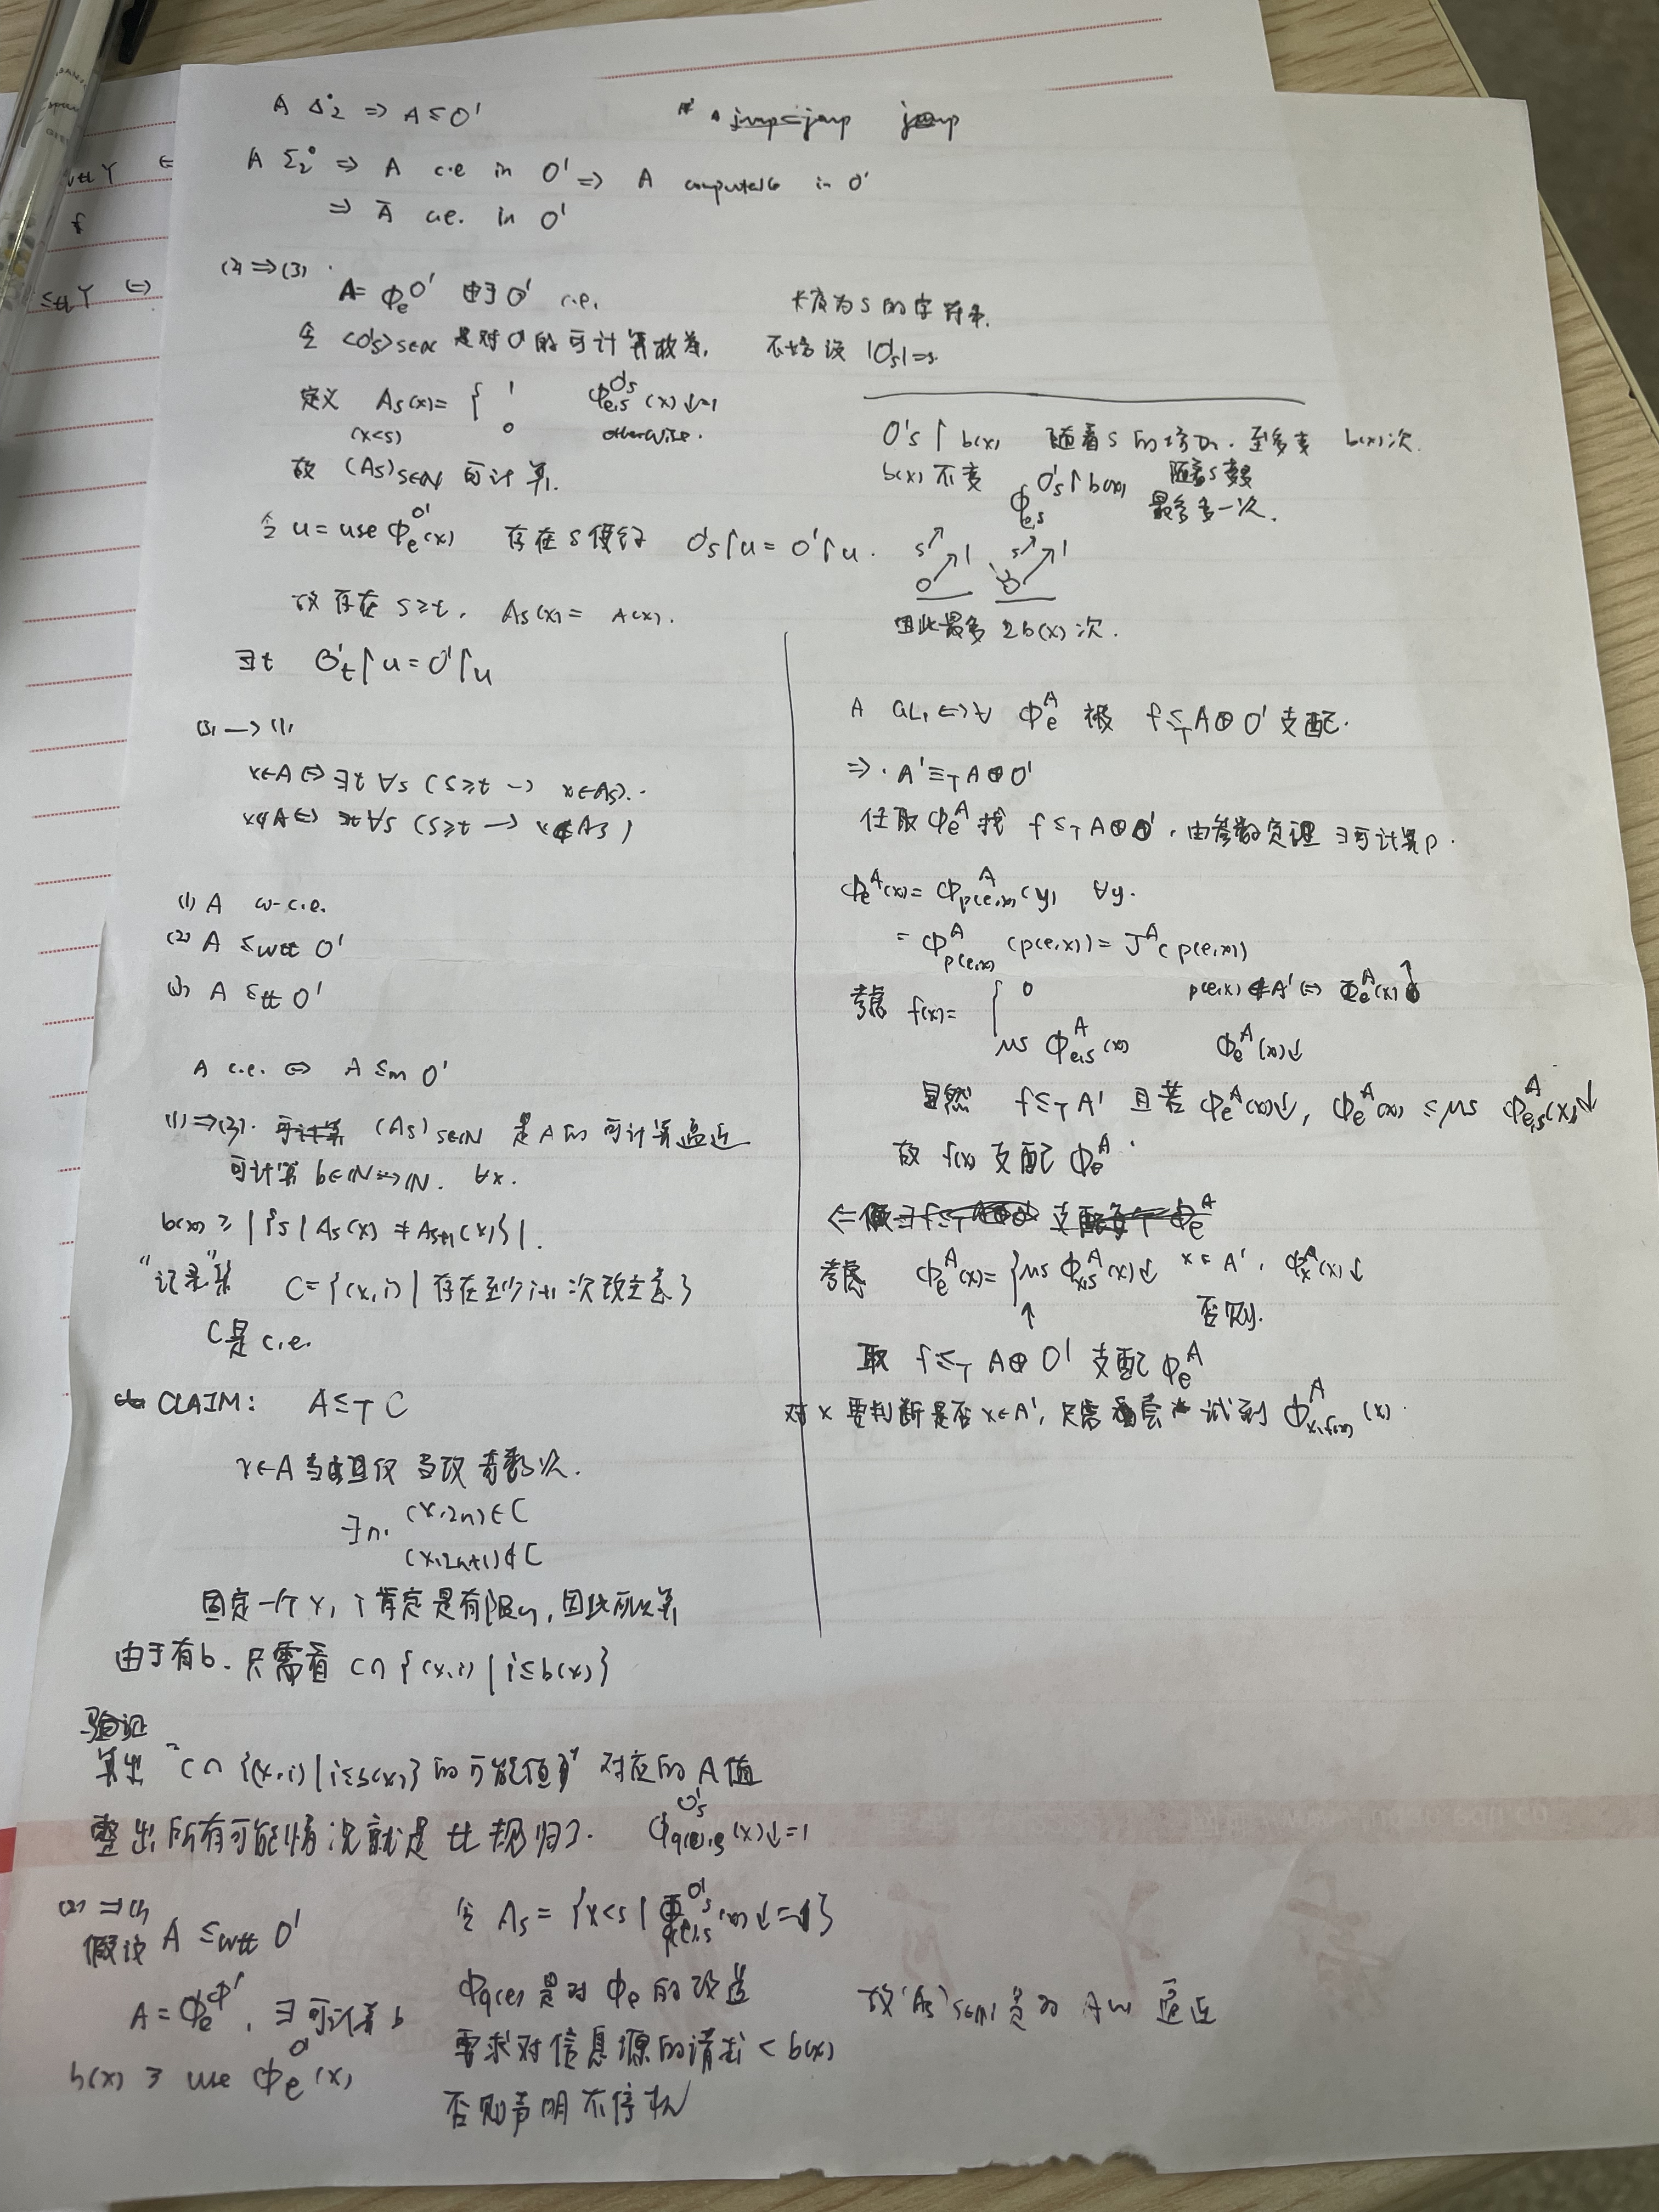
\includegraphics[width=.6\textwidth]{../images/ATourOfC++/1.png}
\label{}
\end{figure}
\section{User-Defined Types}
\label{sec:org2d1de45}
\subsection{Introduction}
\label{sec:org603a9c1}
Types built out of other types using C++’s abstraction mechanisms are called \textbf{user-defined types}.
They are referred to as \textbf{classes} and \textbf{enumerations}.
\subsection{Structures}
\label{sec:org370d6b0}
The \texttt{new} operator allocates memory from an area called the \textbf{free store} (also known as \textbf{dynamic
memory} and \textbf{heap}). Objects allocated on the free store are independent of the scope from which
they are created and ``live'' until they are destroyed using the \texttt{delete} operator
\end{document}
